\documentclass[fleqn]{article}
\usepackage{graphicx}
\usepackage{amsmath,amsfonts,amssymb}
\usepackage{commath}
\usepackage[export]{adjustbox}

\usepackage{titlesec}
\titlelabel{\thetitle)\quad}

\usepackage{changepage,titlesec}
\titleformat{\section}[block]{\bfseries}{\thesection)}{1em}{}
\titleformat{\subsection}[block]{}{(\thesubsection)}{1em}{}
\titleformat{\subsubsection}[block]{}{(\thesubsubsection)}{1em}{}
\titlespacing*{\subsection} {2em}{3.25ex plus 1ex minus .2ex}{1.5ex plus .2ex}
\titlespacing*{\subsubsection} {4em}{3.25ex plus 1ex minus .2ex}{1.5ex plus .2ex}

\usepackage{geometry}
 \geometry{
 a4paper,
 total={170mm,257mm},
 left=20mm,
 top=20mm,
 }

\title{Homework 3}
\author{Submitted By: Puneet Singhal\\ \\ {Collaborated with Abhijeet Chilukuri}}
\date{}

\def\thesubsection{\alph{subsection}}
\def\thesubsubsection{\roman{subsubsection}}

\begin{document}
\maketitle
\pagenumbering{arabic}


\section{ }

\subsection{}
\begin{adjustwidth}{4em}{0pt}
	Point-to-plane: The minimization is done over the sum of squared distances between each source point and the tangent plane at its corresponding destination point. 
	More specifically, if $s_i = (s_{ix}, s_{iy}, s_{iz}, 1)^T$ is a source point, $d_i = (d_{ix}, d_{iy}, d_{iz}, 1)^T$ is the corresponding destination	point, and $n_i = (n_{ix}, n_{iy}, n_{iz}, 0)^T$ is the unit normal vector at $d_i$, then the goal of each ICP iteration is to find $M_{opt}$ such that:
	
	$\\ M_{opt} = \arg \min_M \Sigma_i ((Ms_i - d_i)\boldsymbol{.}n_i)^2 \\$
	
	whereas, in Point-to-point ICP approach, the minimization is over sum of squared distances between the 2 point clouds.
	
\end{adjustwidth}

\subsection{}
\begin{adjustwidth}{4em}{0pt}
	\begin{align}
		\tilde{T}^z_{g,k} &= \tilde{T}^z_{inc} \tilde{T}^{z-1}_{g,k} \\
		\tilde{T}^z_{inc} &= \begin{bmatrix} \tilde{R}^z & \tilde{\boldsymbol{t}}^z\end{bmatrix} \\
		\tilde{T}^z_{g,k} \dot{\boldsymbol{V}}_k(\boldsymbol{u}) &= \tilde{T}^z_{inc} [\tilde{T}^{z-1}_{g,k} \dot{\boldsymbol{V}}_k(\boldsymbol{u})]\\
		& = \begin{bmatrix} \tilde{R}^z & \tilde{\boldsymbol{t}}^z\end{bmatrix} \tilde{\boldsymbol{V}}^g_k(\boldsymbol{u}) \\
		& =  \tilde{R}^z \tilde{\boldsymbol{V}}^g_k(\boldsymbol{u}) + \tilde{\boldsymbol{t}}^z \\
		& = \bigg(\begin{bmatrix} 0 & \alpha & -\gamma \\ -\alpha & 0 & \beta\\ \gamma & -\beta & 0\end{bmatrix} +\boldsymbol{I}_{3 \times 3}\bigg)\tilde{\boldsymbol{V}}^g_k(\boldsymbol{u}) + \tilde{\boldsymbol{t}}^z \\
		& = \bigg(\begin{bmatrix} 0 & \alpha & -\gamma \\ -\alpha & 0 & \beta\\ \gamma & -\beta & 0\end{bmatrix}\tilde{\boldsymbol{V}}^g_k(\boldsymbol{u}) + \boldsymbol{I}_{3 \times 3} \times \tilde{\boldsymbol{t}}^z+ \tilde{\boldsymbol{V}}^g_k(\boldsymbol{u}) \\
		& = \big[\tilde{\boldsymbol{V}}^g_k(\boldsymbol{u})\big]_X \begin{bmatrix} \beta \\ \gamma \\ \alpha \end{bmatrix} + \boldsymbol{I}_{3 \times 3} \begin{bmatrix} t_x \\ t_y \\ t_z \end{bmatrix}+ \tilde{\boldsymbol{V}}^g_k(\boldsymbol{u}) \\
		& = \bigg[\big[\tilde{\boldsymbol{V}}^g_k(\boldsymbol{u})\big]_X + \boldsymbol{I}_{3 \times 3}\bigg] \begin{bmatrix} \beta & \gamma & \alpha & t_x & t_y & t_z \end{bmatrix}^T + \tilde{\boldsymbol{V}}^g_k(\boldsymbol{u}) \\
		& = \bigg[\big[\tilde{\boldsymbol{V}}^g_k(\boldsymbol{u})\big]_X + \boldsymbol{I}_{3 \times 3}\bigg] \boldsymbol{X} + \tilde{\boldsymbol{V}}^g_k(\boldsymbol{u}) \\
	\end{align}	
\end{adjustwidth}


\subsection{}
\begin{adjustwidth}{4em}{0pt}
	MATLAB functions updated
\end{adjustwidth}


\subsection{}
\begin{adjustwidth}{4em}{0pt}
	Number of points in the final model = 1063659 \newline
	Compression ratio = 13.32  \newline
	Total time spent = 13.25 sec \newline
	\newline \newline
	The images shows that the although the features like painting, couch, pillows, cushions etc are being captured, some of them are more accurate than other. For example, the right side of couch is still not mapped correctly, we can see some points going towards right. \\
	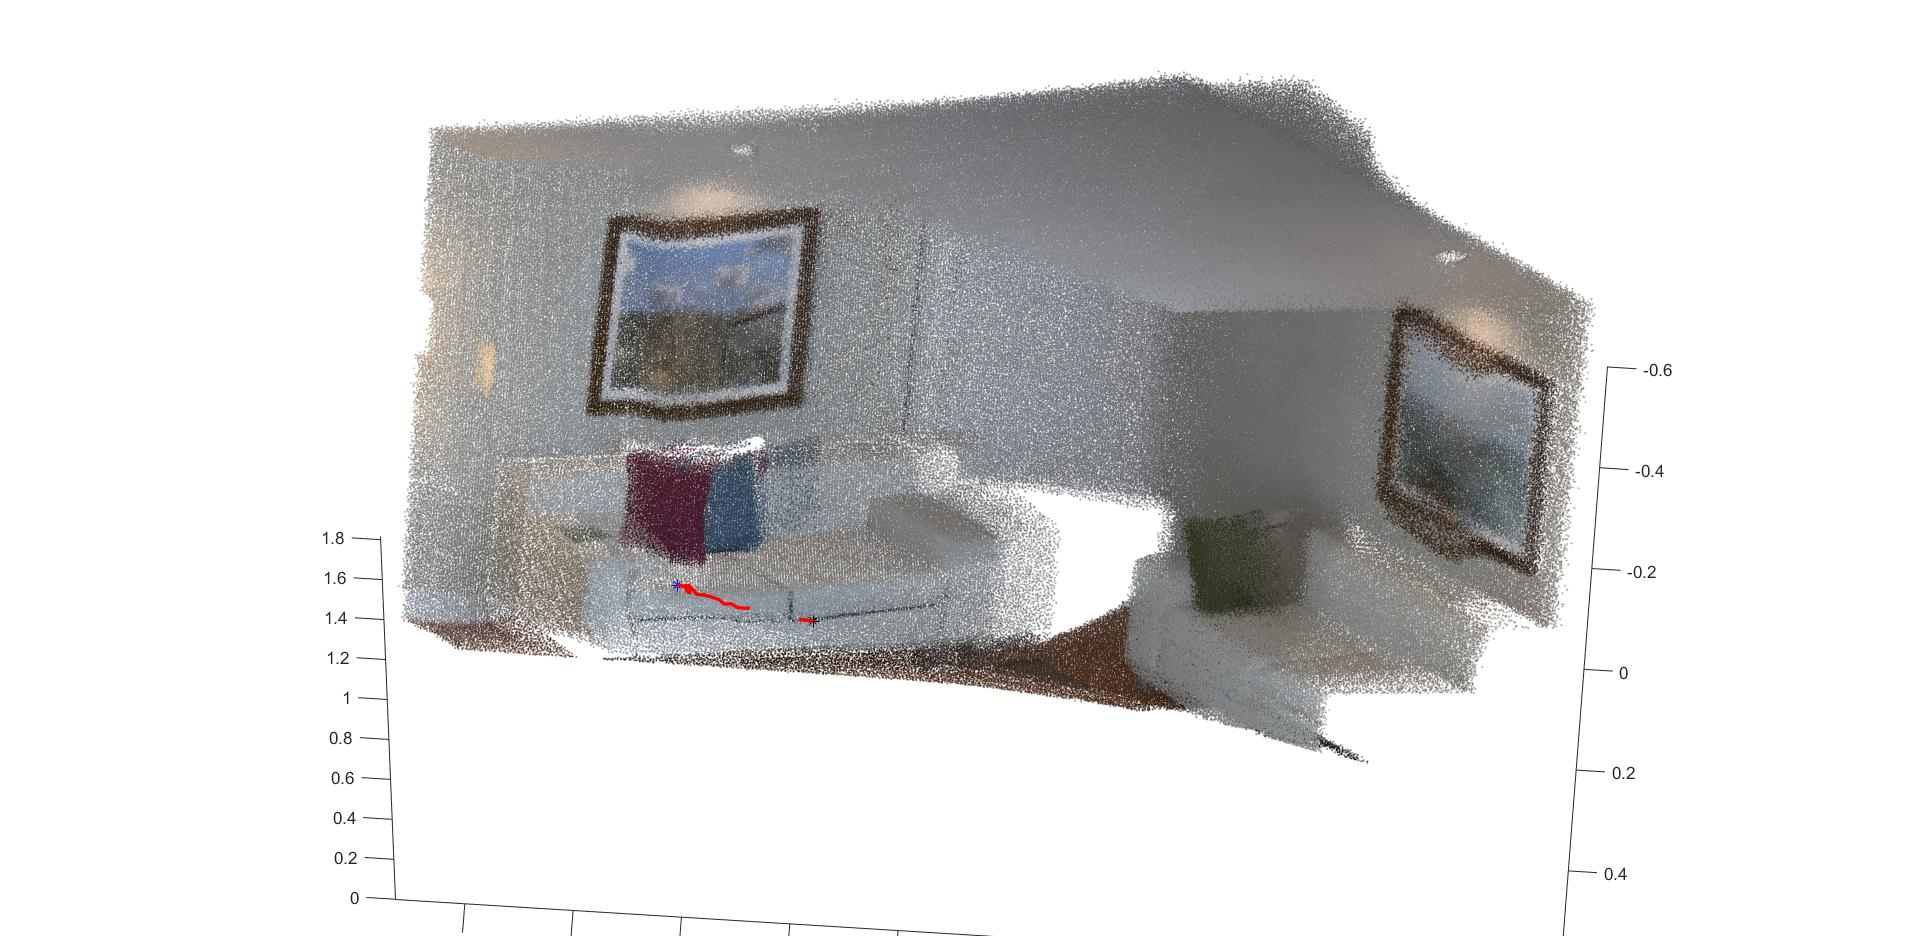
\includegraphics[width = 1\textwidth,center]{slam_hw3_q1_d_pic1.jpg}\\ \\
	Additionally, not all points are close to their truth value leading to different depths and hence bending effect in the image as can be deduced from frame in below picture.\\
	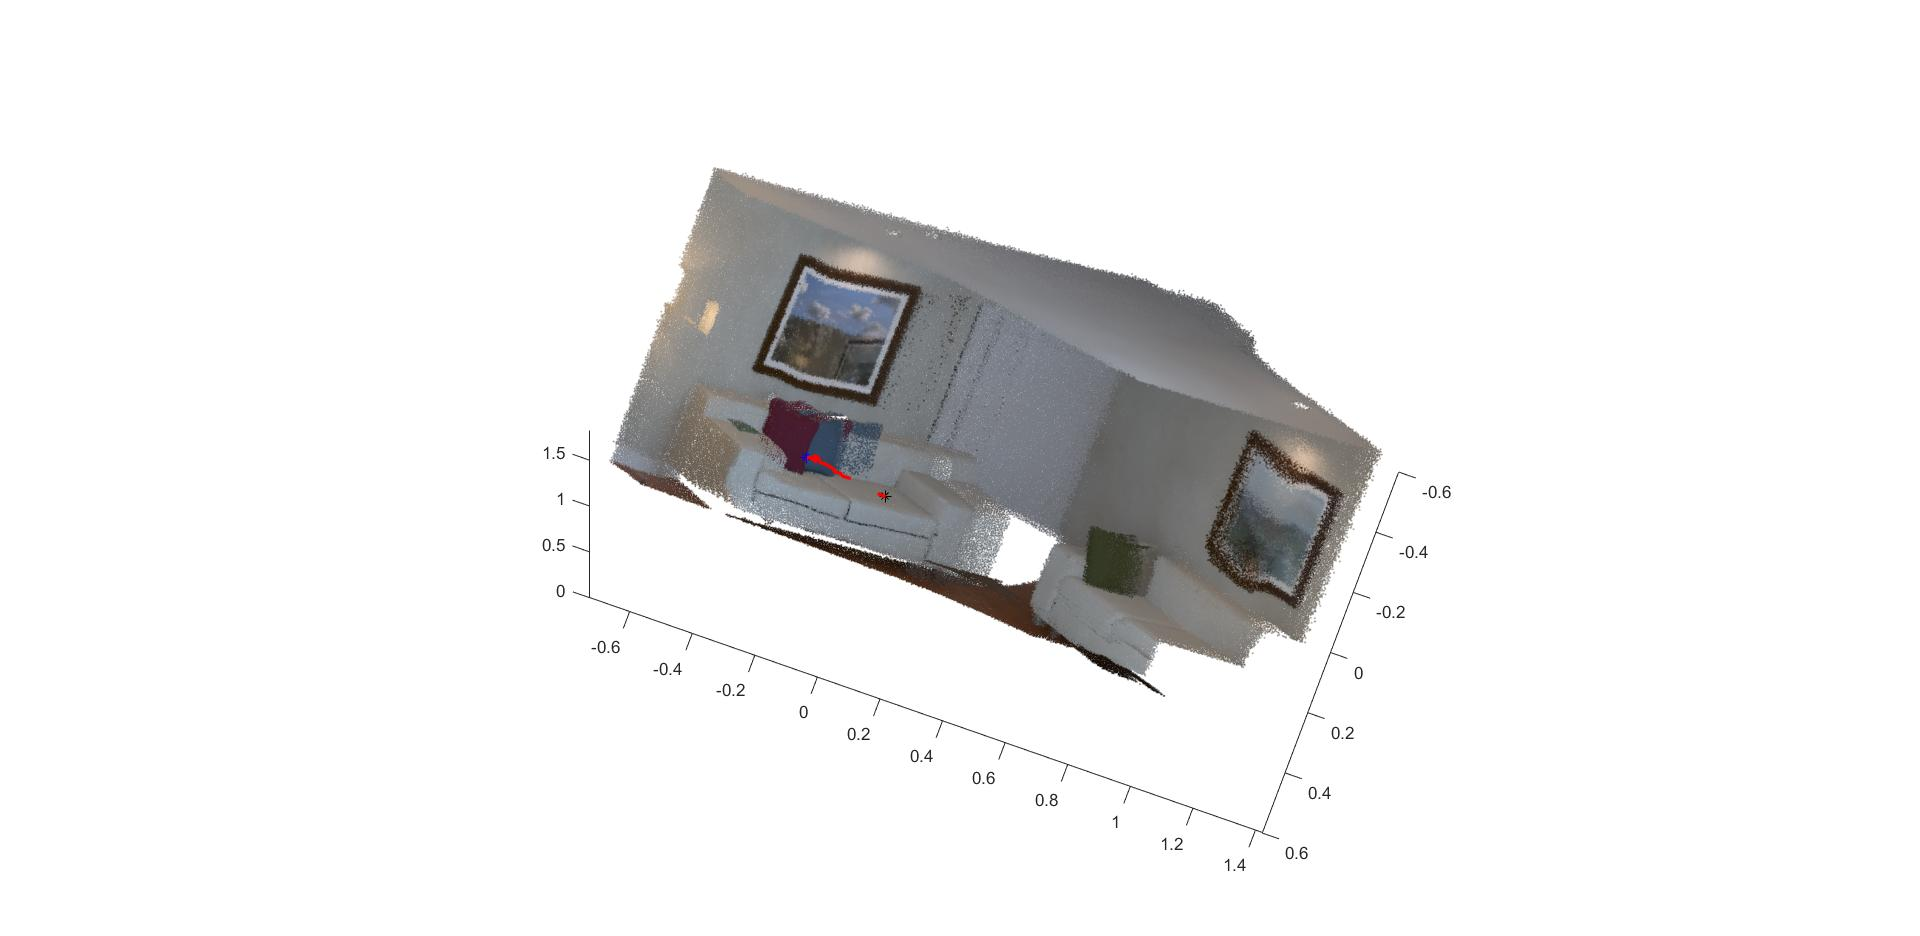
\includegraphics[width = 1.5\textwidth,center]{slam_hw3_q1_d_pic2.jpg}\\ \\
	Some of the portion of the room is not captured which might be due to occlusions like corner between 2 couches and right ends of pillow. Also the camera tracking is not continuous and breaks at one point. \\
	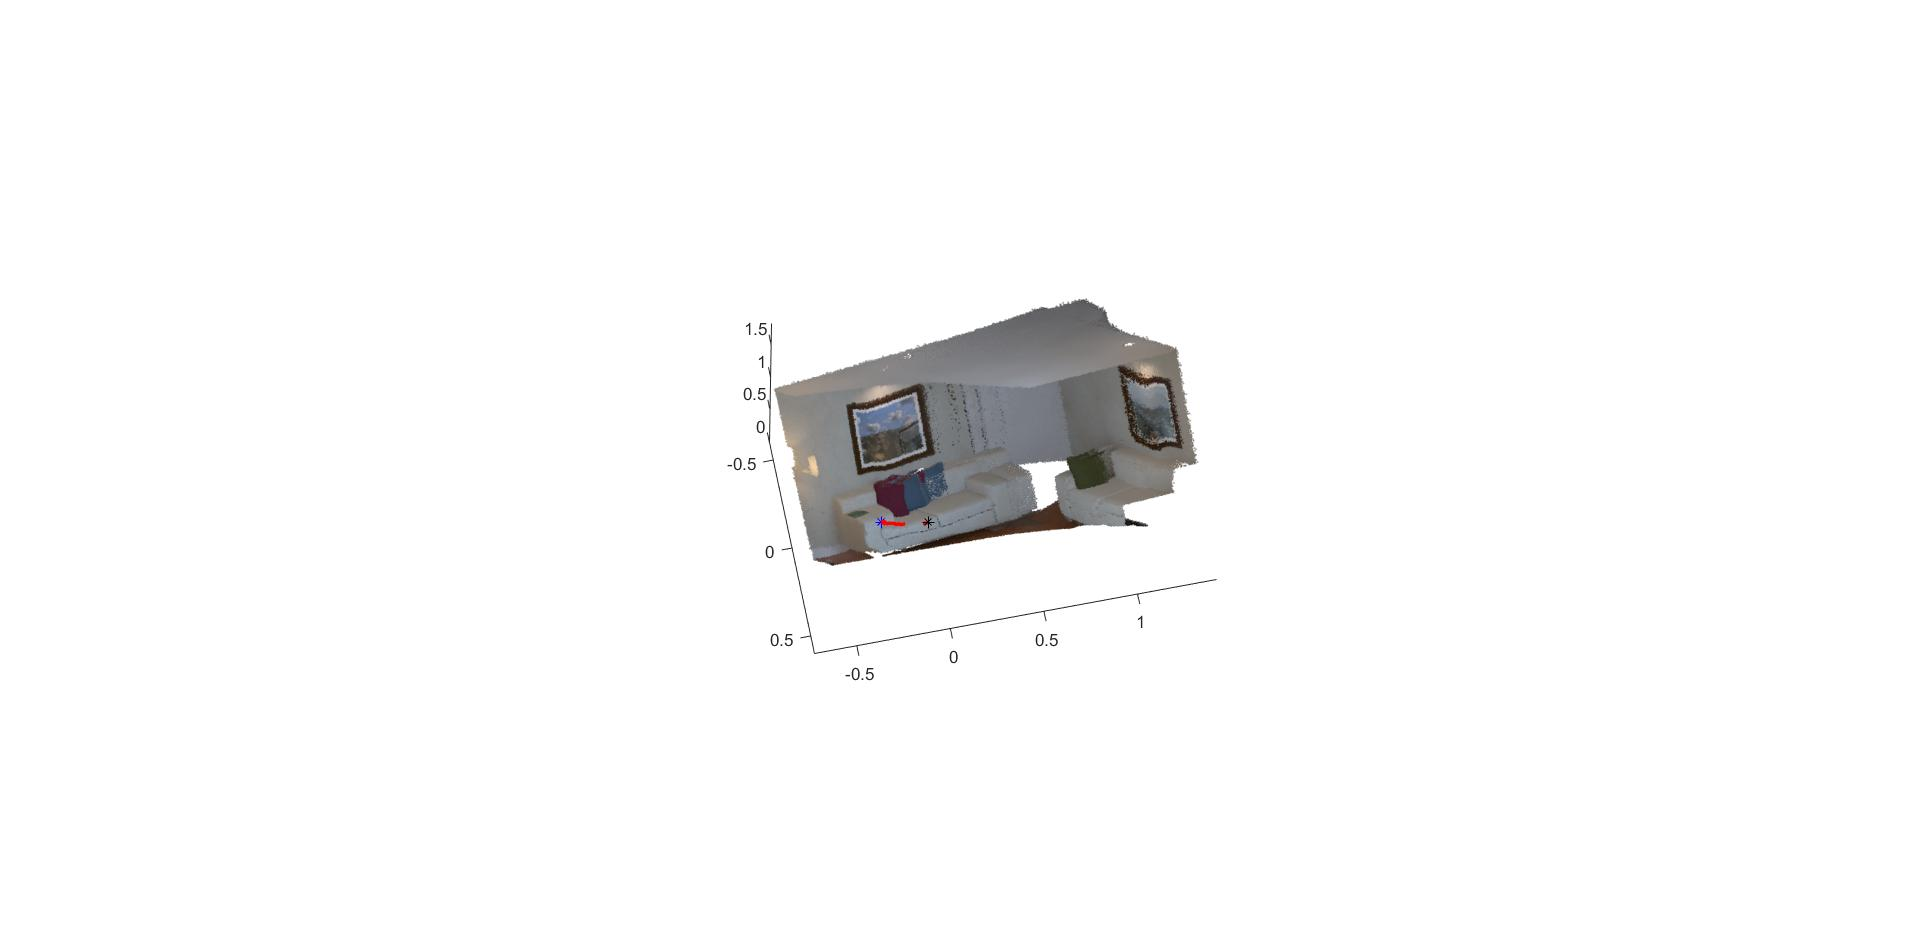
\includegraphics[width = 2.5\textwidth,center]{slam_hw3_q1_d_pic3.jpg}\\ \\
	
\end{adjustwidth}

\section{}
\subsection{}
\begin{adjustwidth}{4em}{0pt}
	The volumetric fusion method of supports incremental updates, exploits redundant samples, makes no topological assumptions, approximates sensor uncertainty, and fusion is performed using a simple weighted average. For active sensors, this method produces very compelling results [2, 9, 6, 11]. The
	drawbacks are: \newline
	1.) the \itshape{computational overheads} needed to continuously transition between different data representations, where point-based input is converted to a continuous implicit function, discretized within a regular grid data structure, and converted back to an (explicit) form using expensive polygonization or raycasting methods. \newline
	2.) the \itshape{memory overheads} imposed by using a regular voxel grid, which represents both empty space and surfaces densely, and thus greatly limits the size of reconstruction volume. \newline
	
	Point-based representations are more amenable to the input acquired from depth/range sensors.\newline
	
	Beyond reducing computational complexity, point-based methods lower the memory overhead associated with volumetric (regular grid) approaches, as long as overlapping points are merged.
	
\end{adjustwidth}

\subsection{}
\begin{adjustwidth}{4em}{0pt}
	$\boldsymbol{n'} = R\boldsymbol{n}$
\end{adjustwidth}

\subsection{}
\begin{adjustwidth}{4em}{0pt}
	MATLAB functions updated
\end{adjustwidth}


\subsection{}
\begin{adjustwidth}{4em}{0pt}
	Number of points in the final model = 1344457 \newline
	Compression ratio = 16.83 \% \newline
	Total time spent = 27.51 sec \newline
	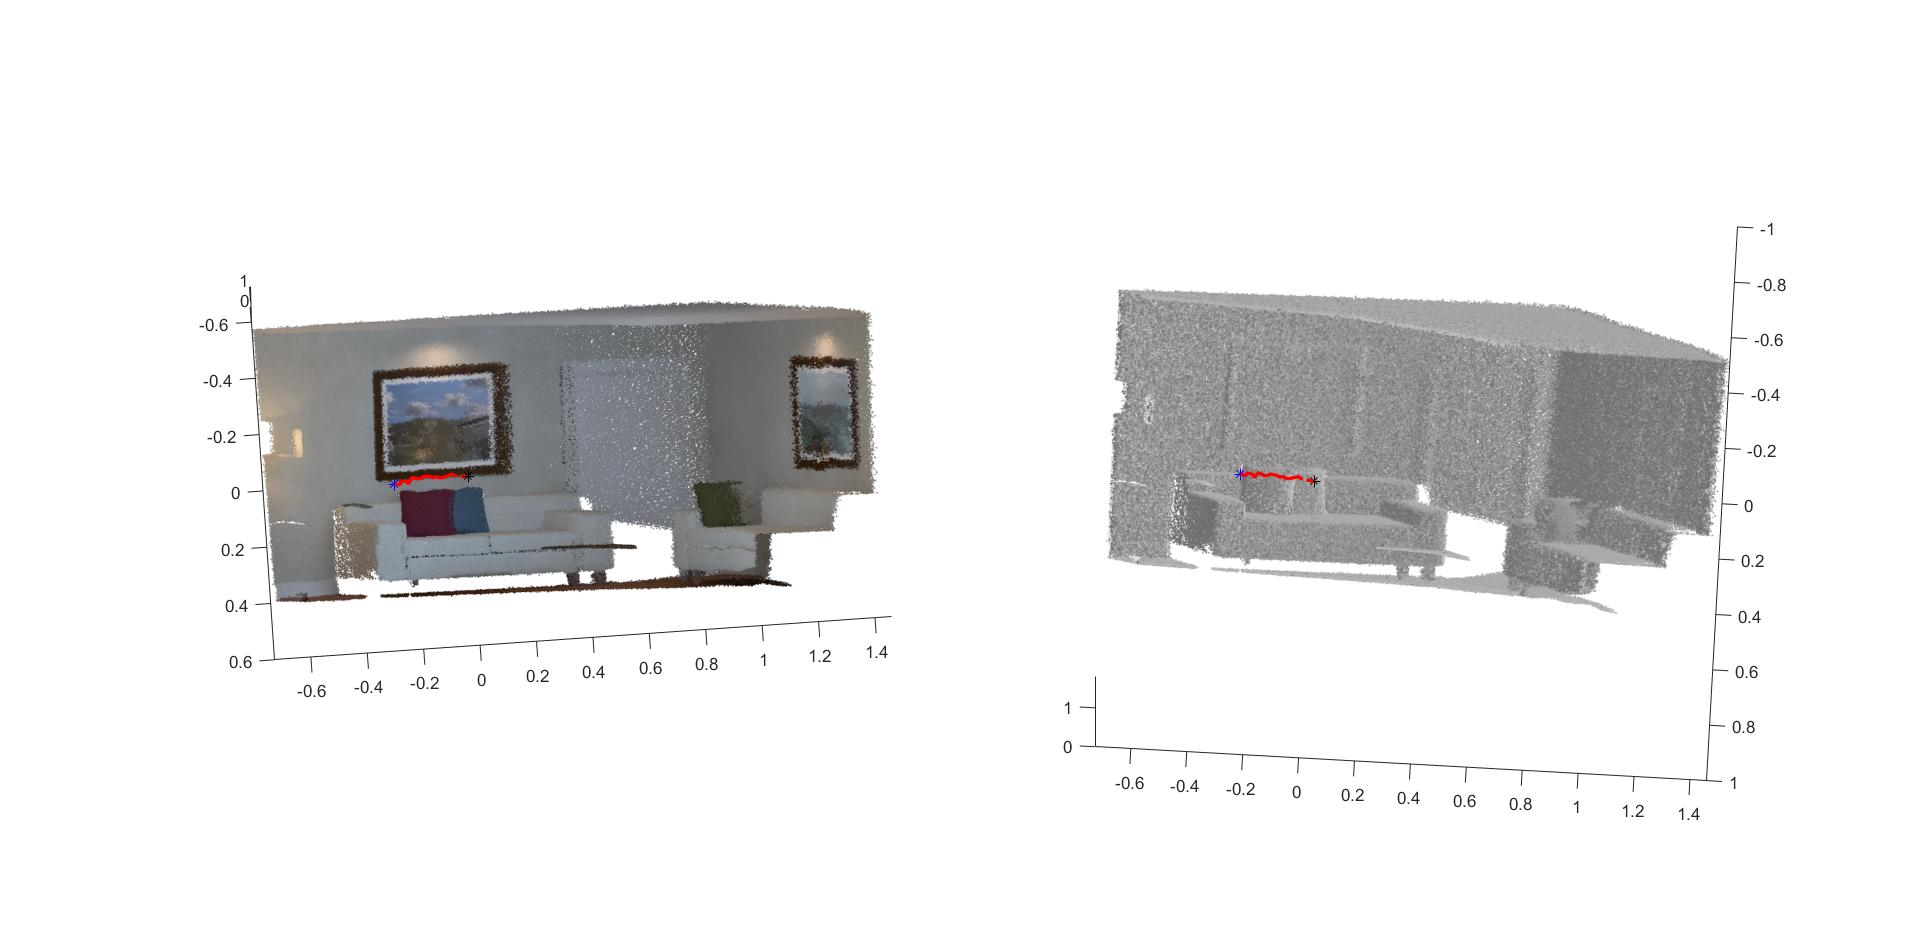
\includegraphics[width = 1.25\textwidth,center]{slam_hw3_q2_d_part1_pic1.jpg}\\ \\
	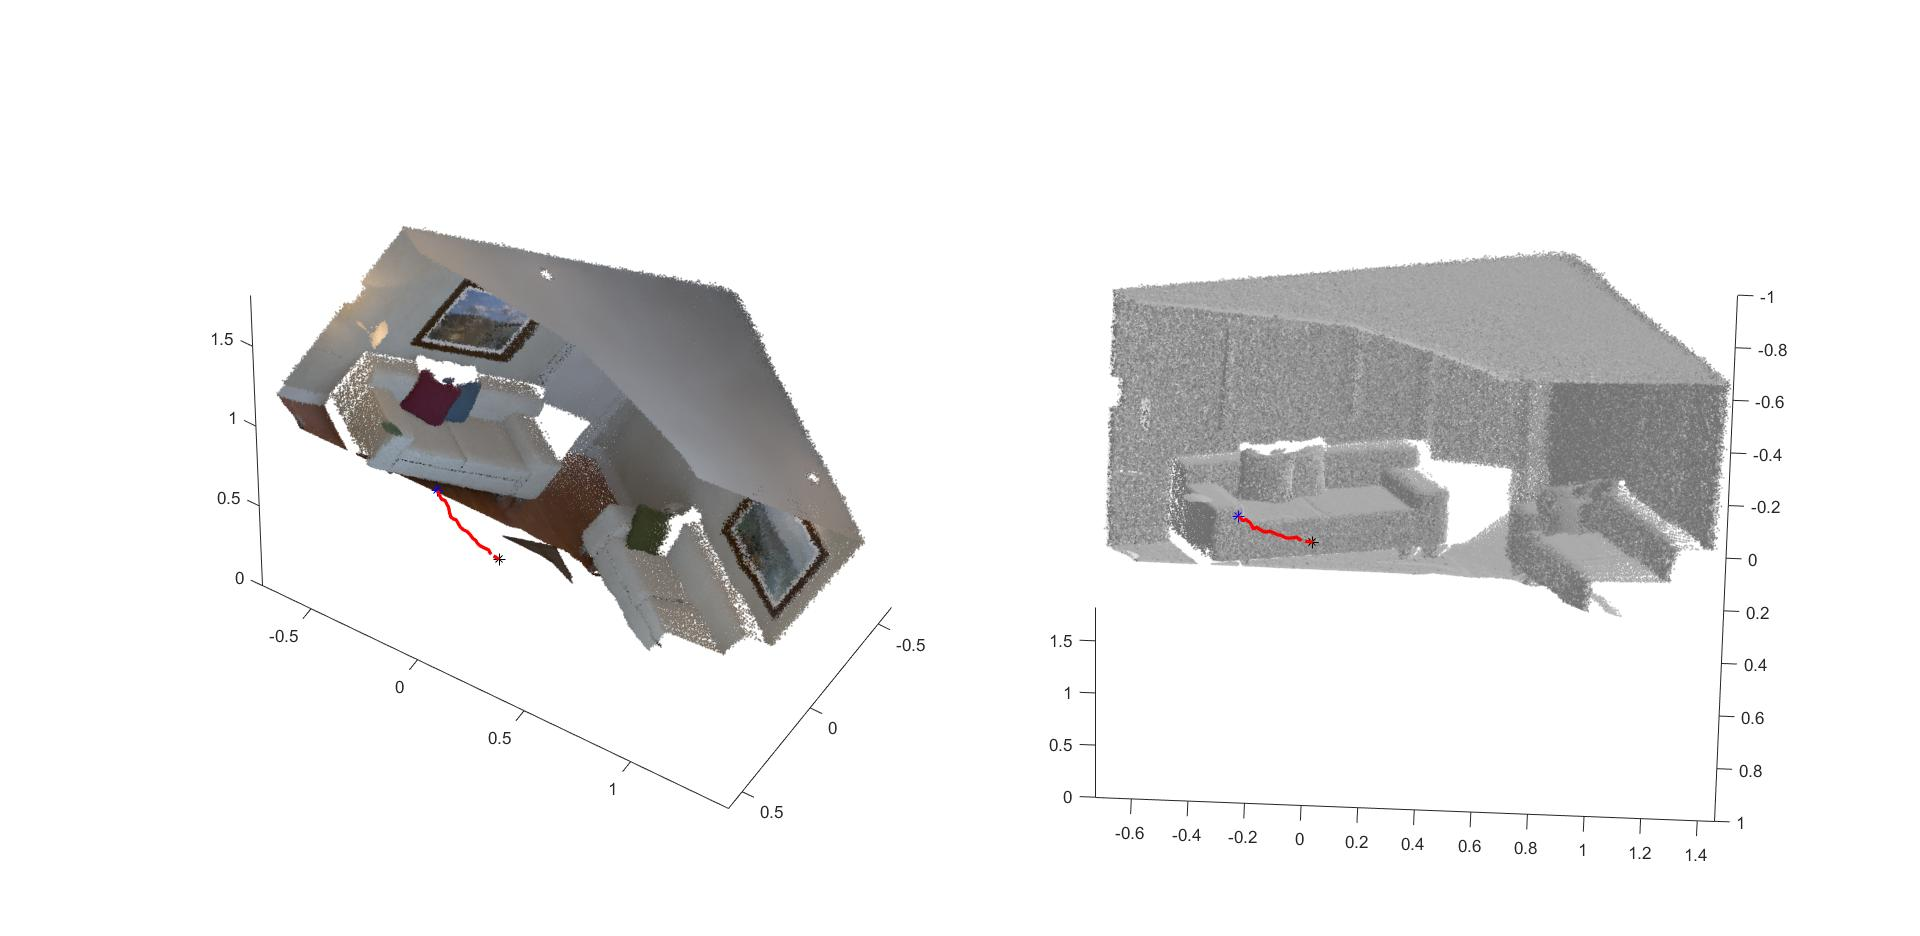
\includegraphics[width = 1.25\textwidth,center]{slam_hw3_q2_d_part1_pic2.jpg}\\ \\
	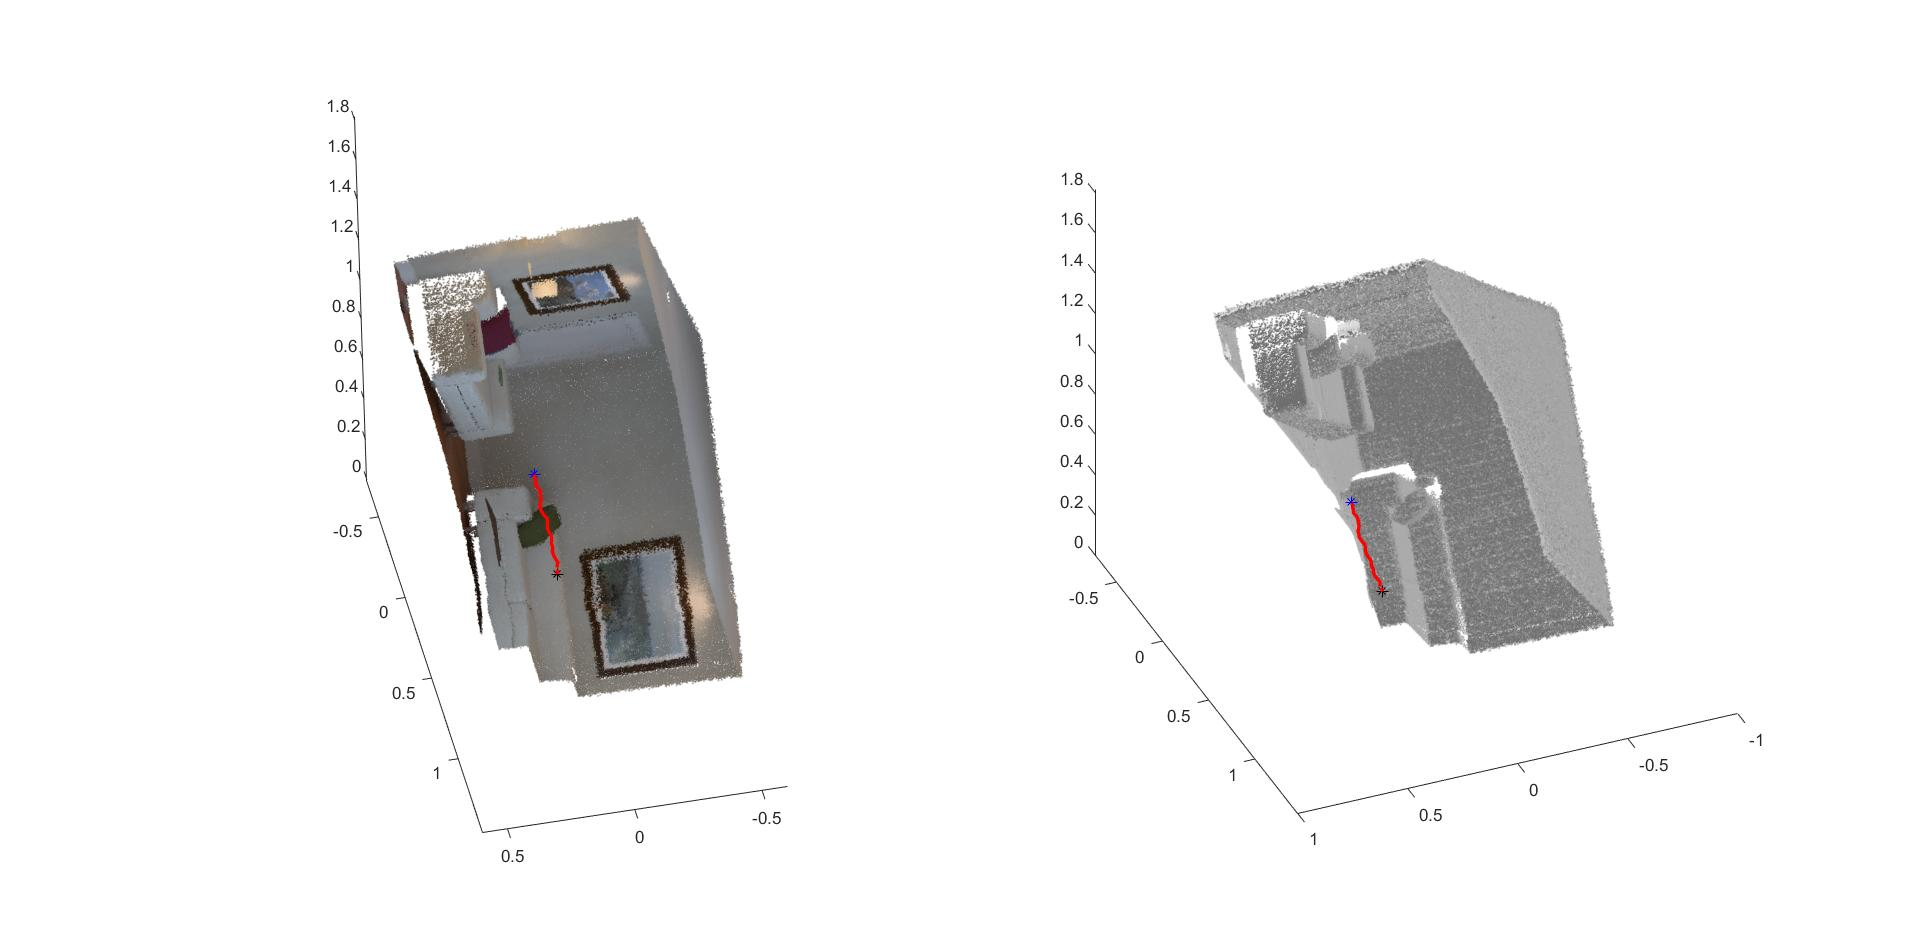
\includegraphics[width = 1.25\textwidth,center]{slam_hw3_q2_d_part1_pic3.jpg}\\ \\
	\newline \newline
	
	If is\_debug\_fusion is set to 1: \newline
	Number of points in the final model = 1360511 \newline
	Compression ratio = 17.03 \% \newline
	Total time spent = 27.01 sec \newline
	Camera tracking is still breaking but for a shorter duration as compared with results from last question. \\
	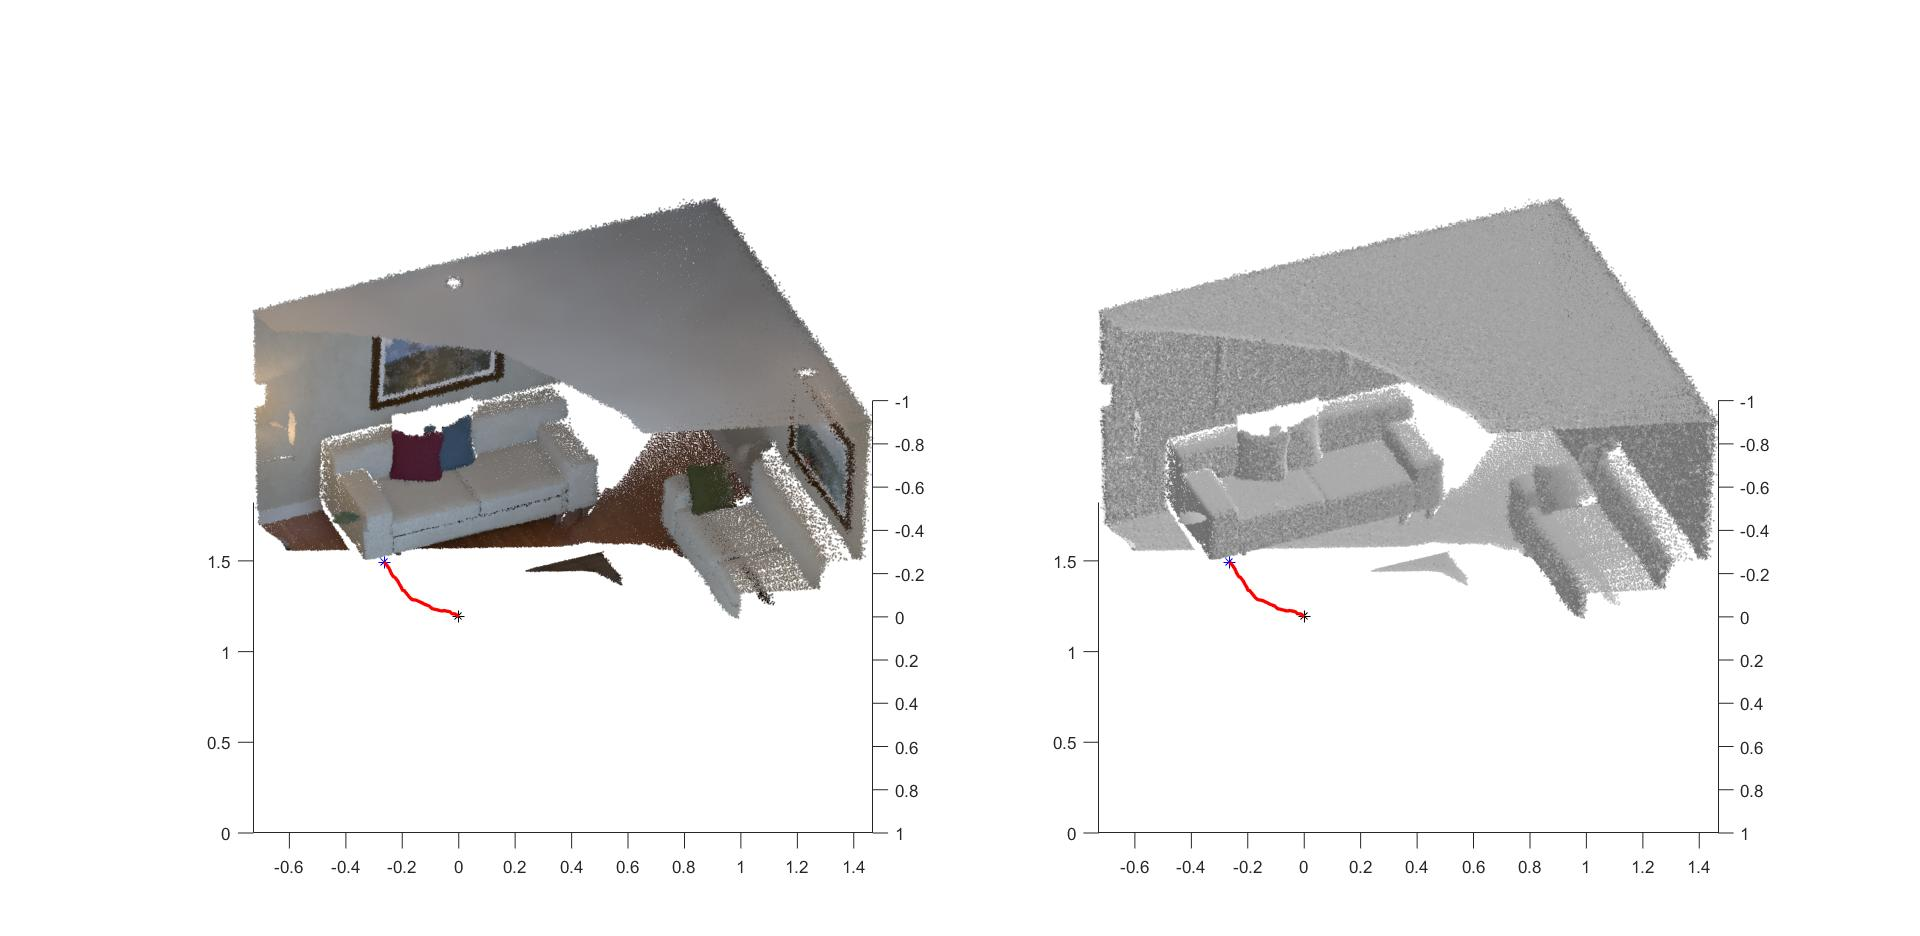
\includegraphics[width = 1\textwidth,center]{slam_hw3_q2_d_part2_pic1.jpg}\\
	The map is certainly more densed capturing more information and improving features. For example, the end of couch are not dispersing and are properly mapped.\\
	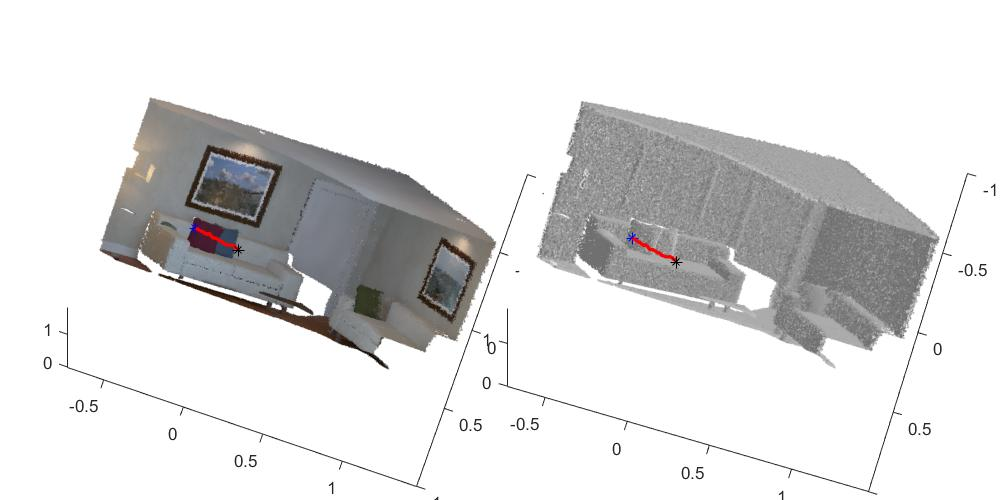
\includegraphics[width = 1\textwidth,center]{slam_hw3_q2_d_part2_pic2.jpg}\\ \\
	The positions are more close to truth values and shifting of points/distortion of features has reduced by significant amount. This can be observed by looking at left painting; the edges are not distorted compared to previous question where they were hugely distorted \\
	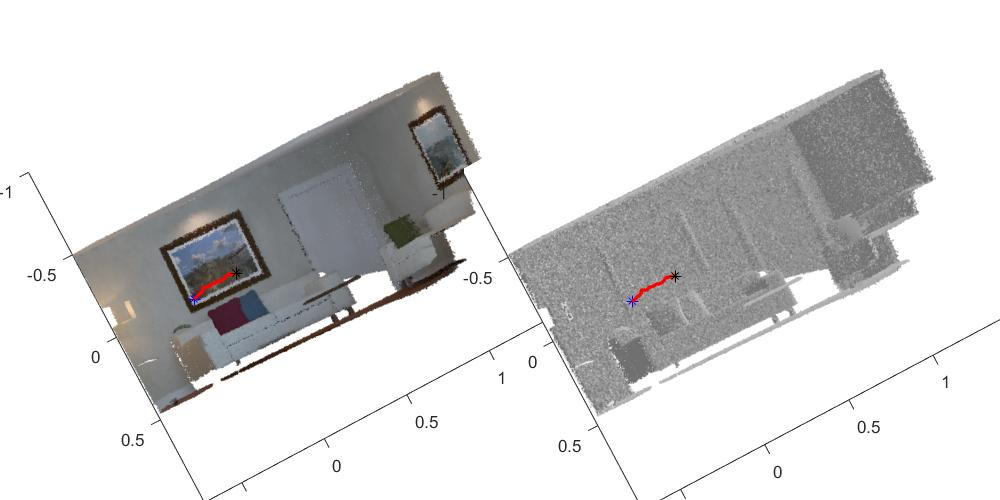
\includegraphics[width = 1\textwidth,center]{slam_hw3_q2_d_part2_pic3.jpg}\\ \\
	
\end{adjustwidth}

\section{}
\subsection{}
\begin{adjustwidth}{4em}{0pt}
	Using fusion model as the next reference frame results in better ICP registration than using current frame because the current frame captures points at that instance only whereas, by using fusion model, we essentially consider the points captured till now and make them available in next iteration. This increases the number of inliers (at least same inliers compared to the case using current frame as reference) which improves the performance of the algorithm.
	
\end{adjustwidth}

\subsection{}
\begin{adjustwidth}{4em}{0pt}
	Number of inliers tell us the number of points that got associated between reference points and input points. More the inliers implies more association which implies small change in frame which is important for small angle assumptions. Also, assuming slow motion of camera, more inliers implies that the more points are getting updated showing better performance in pointcloud registration.
	Similar explanation goes for RMSE as low error signifies that the points are very close to each other which means that pointcloud is getting rightly registered. \newline
	
	More the compression ratio more is the number of points in te output of fusion map for given input sequence. We would want the output to be very dense and hence higher compression ratio is desired.
\end{adjustwidth}

\subsection{}
\begin{adjustwidth}{4em}{0pt}
	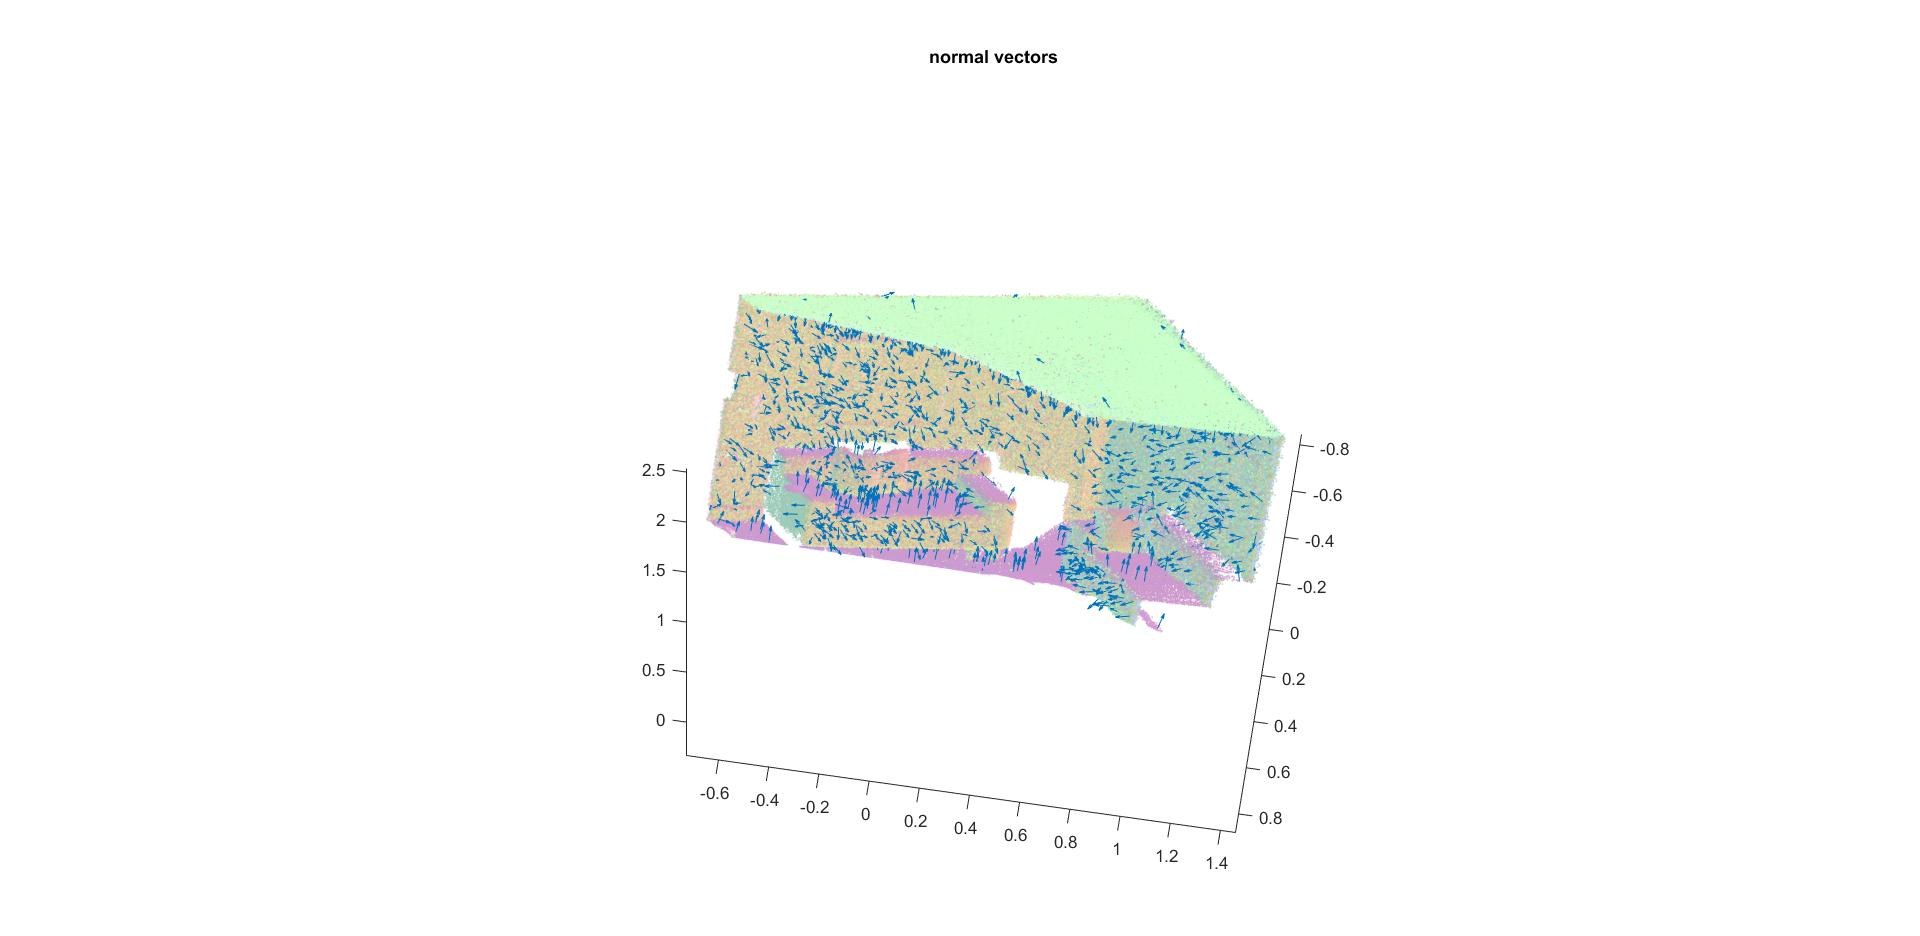
\includegraphics[width = 1.5\textwidth,center]{slam_hw3_q3_partc_normalVectors.jpg}\\
	The arrows respresent surface normals of the points in fusion map. It can be observed that the direction of arrows are very close to the normals of the surfaces like the top of the roof but some of the normals are not as close and have errors like side walls.
	
	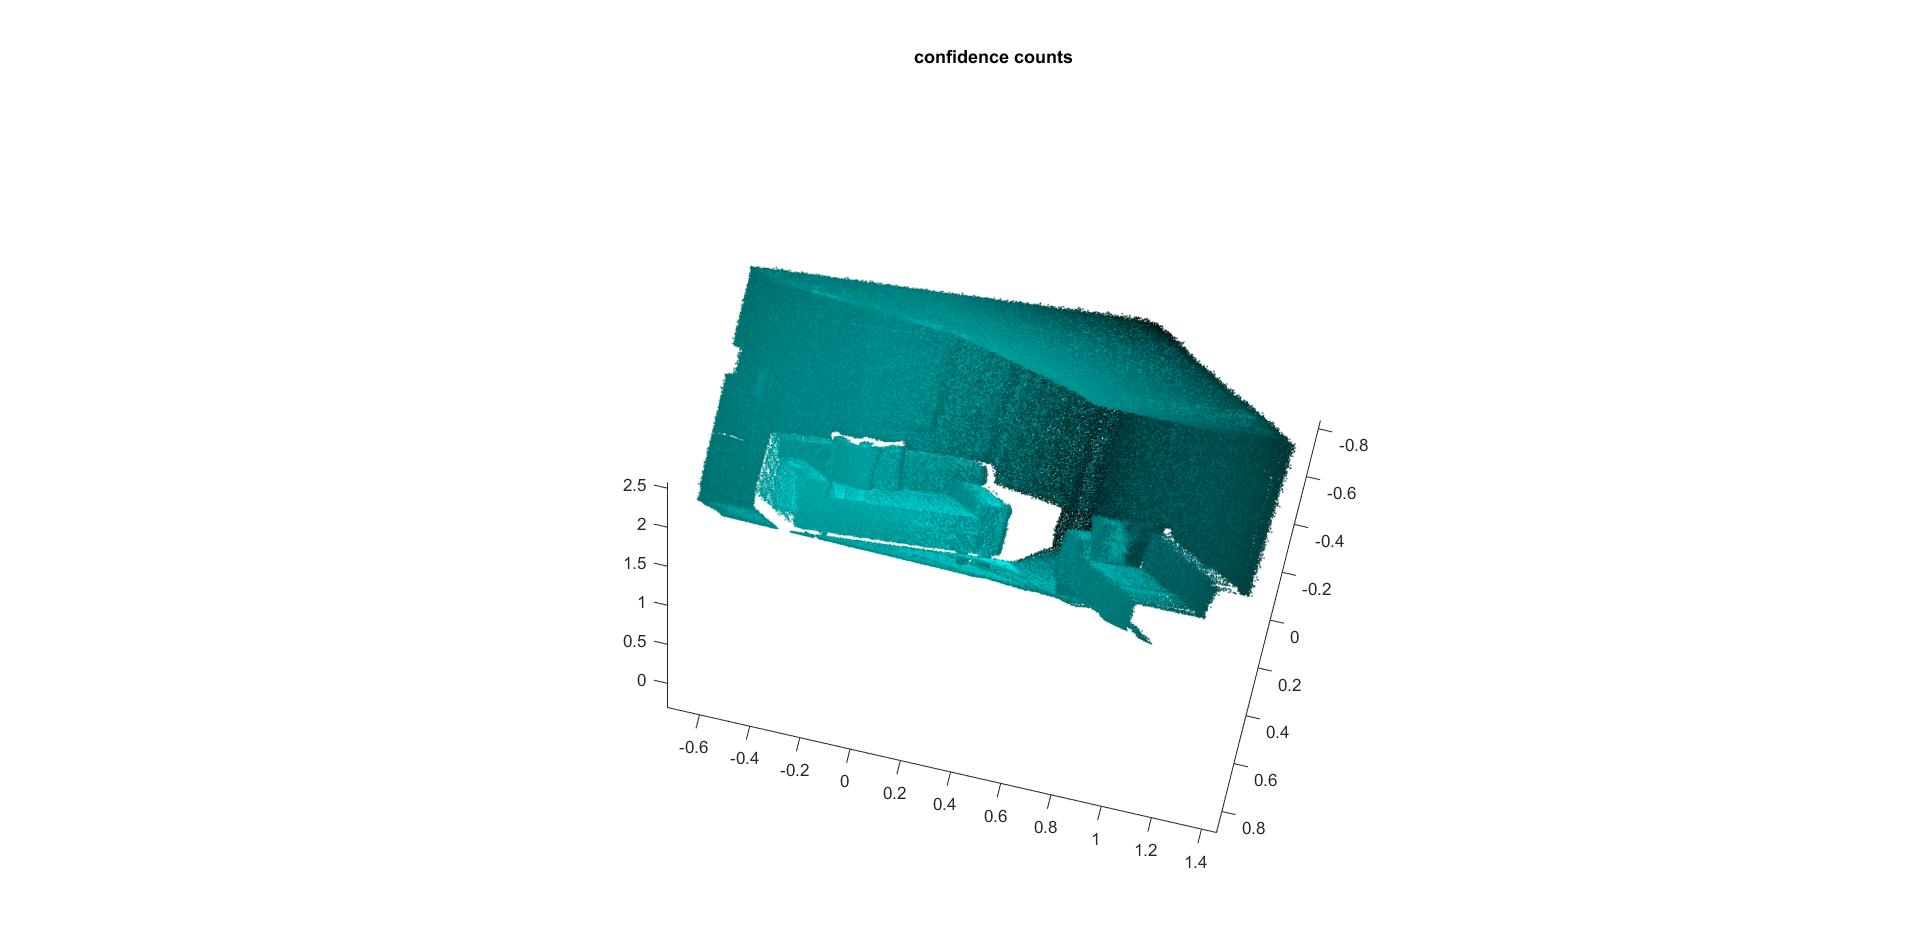
\includegraphics[width = 1.5\textwidth,center]{slam_hw3_q3_partc_confidenceCounts.jpg}\\
	In the figure, dark color represents the points that were not updated much and hence there is lower confidence count. We would generally remove these points as these are considered unstable points. 
	
	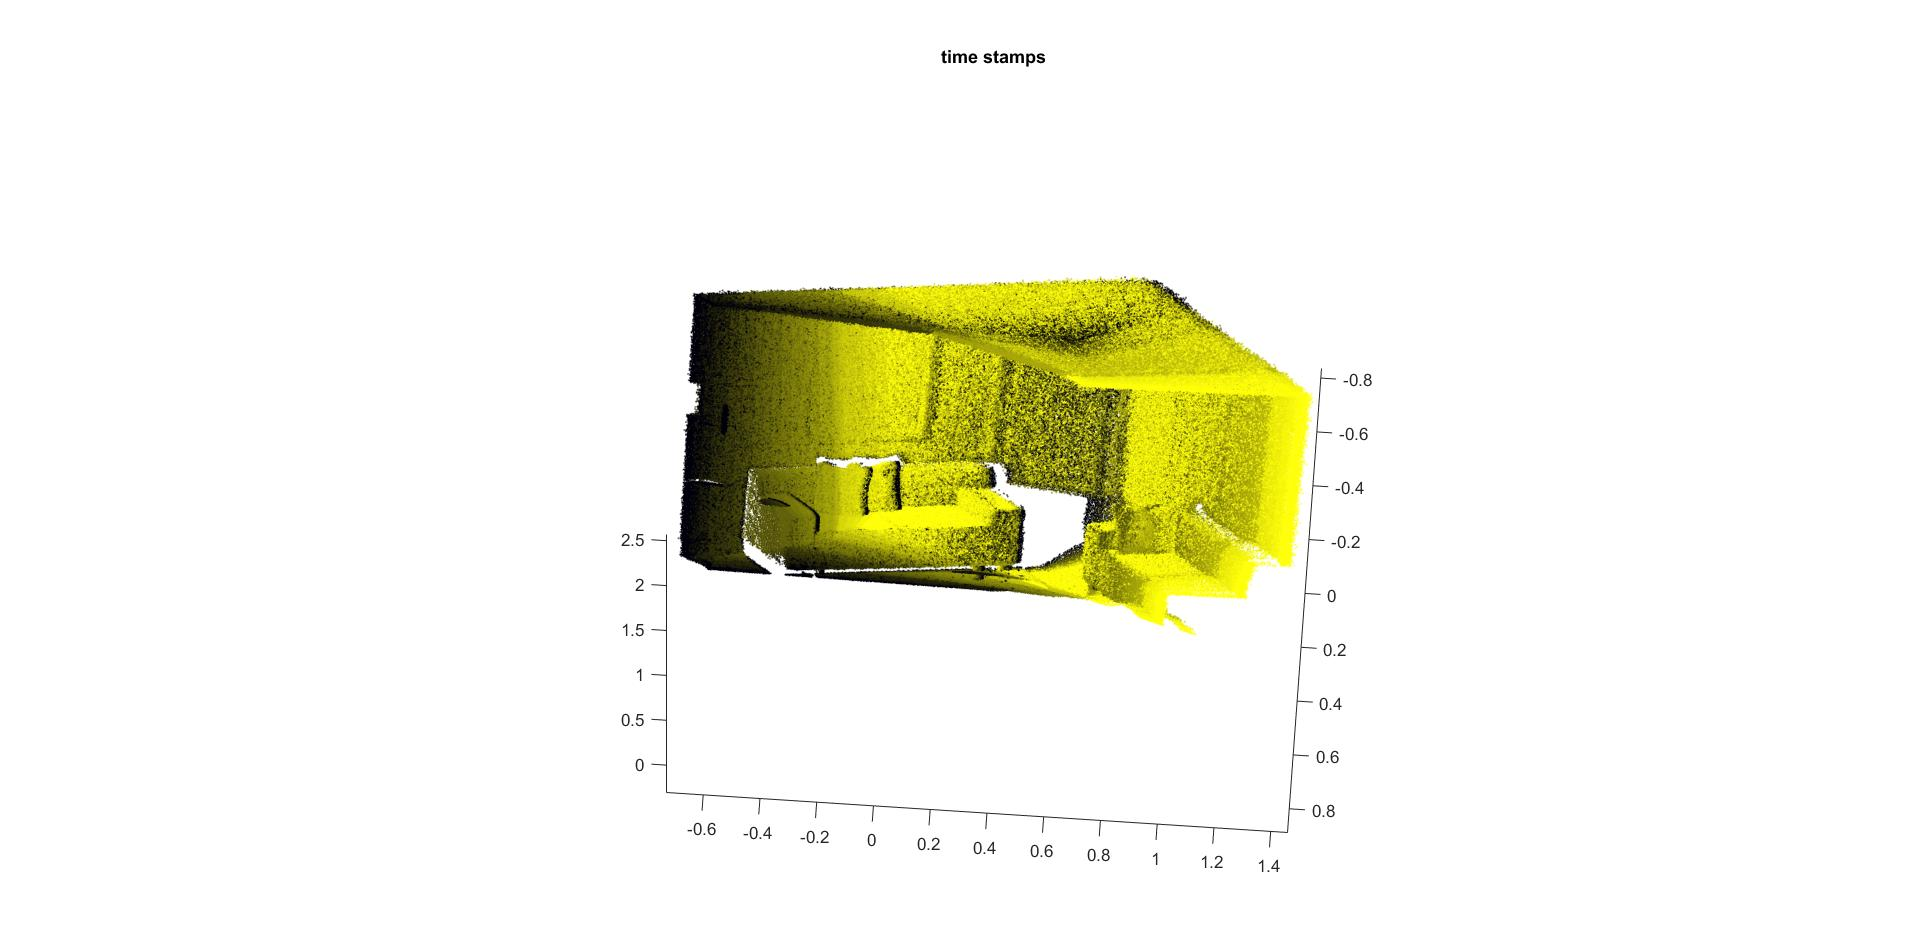
\includegraphics[width = 1.5\textwidth,center]{slam_hw3_q3_partc_timeStamps.jpg}\\
	In the figure, dark color represents the points that were not updated for long time which implies that the correspondence were not found for these points. Thi smight be due to the occlusions which camera was not able to capture during motion like coreners of painting, corners of pillows and other corners. We technically remove the points which were not updated for time $t_{max}$.
\end{adjustwidth}
	
\subsection{}
\begin{adjustwidth}{4em}{0pt}
	To improve the performance, I am removing the points based two criteria in every frame update:\\
	1.) Confidence: Remove the points for which confidence count is less than $C_{Stable} = 0.01$. The value of $C_{Stable}$ is selected as 10 in the paper but here due to very less frames I am choosing small value to show the impact.\\
	2.) Time: remove the points which are not stable for time more than $T_{max}$. the value selected here is 25 but can be optimized.\\
	Results:\\
	Number of points in the final model = 1192487 \\
	Compression ratio = 14.93 \% \\ 
	Total time spent = 28.88 sec \\
	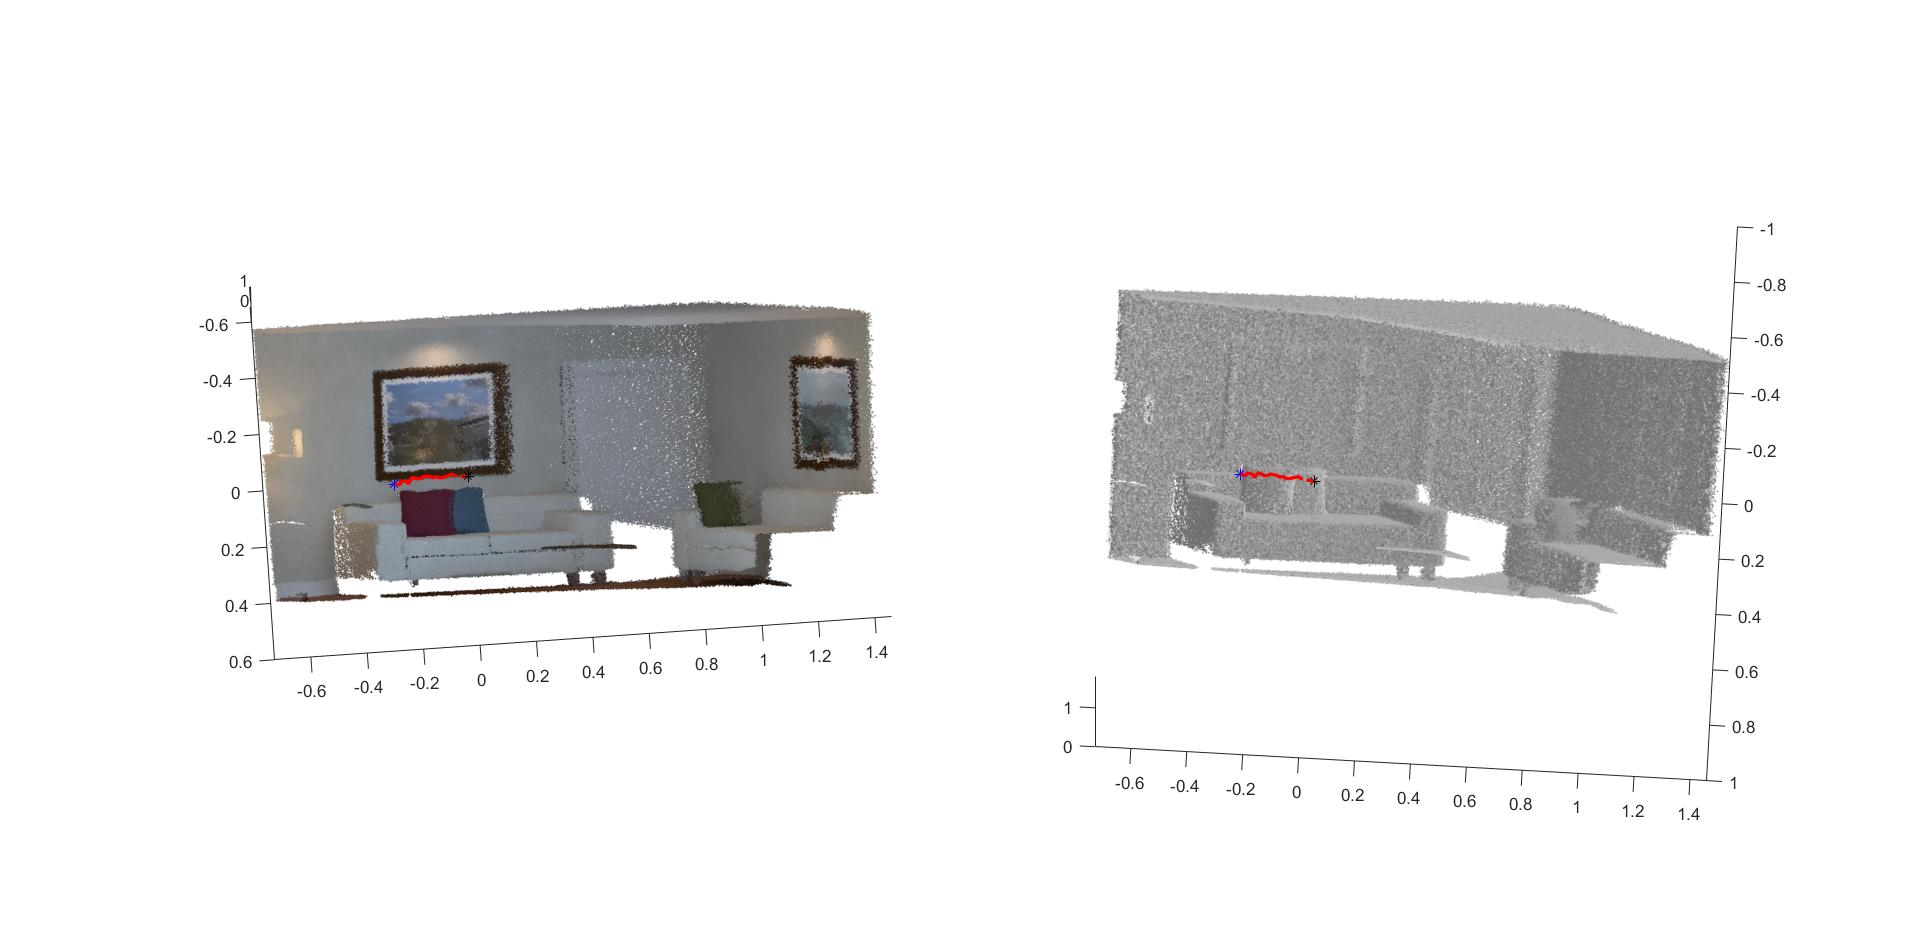
\includegraphics[width = 1.25\textwidth,center]{slam_hw3_q2_d_part1_pic1.jpg}\\ \\
	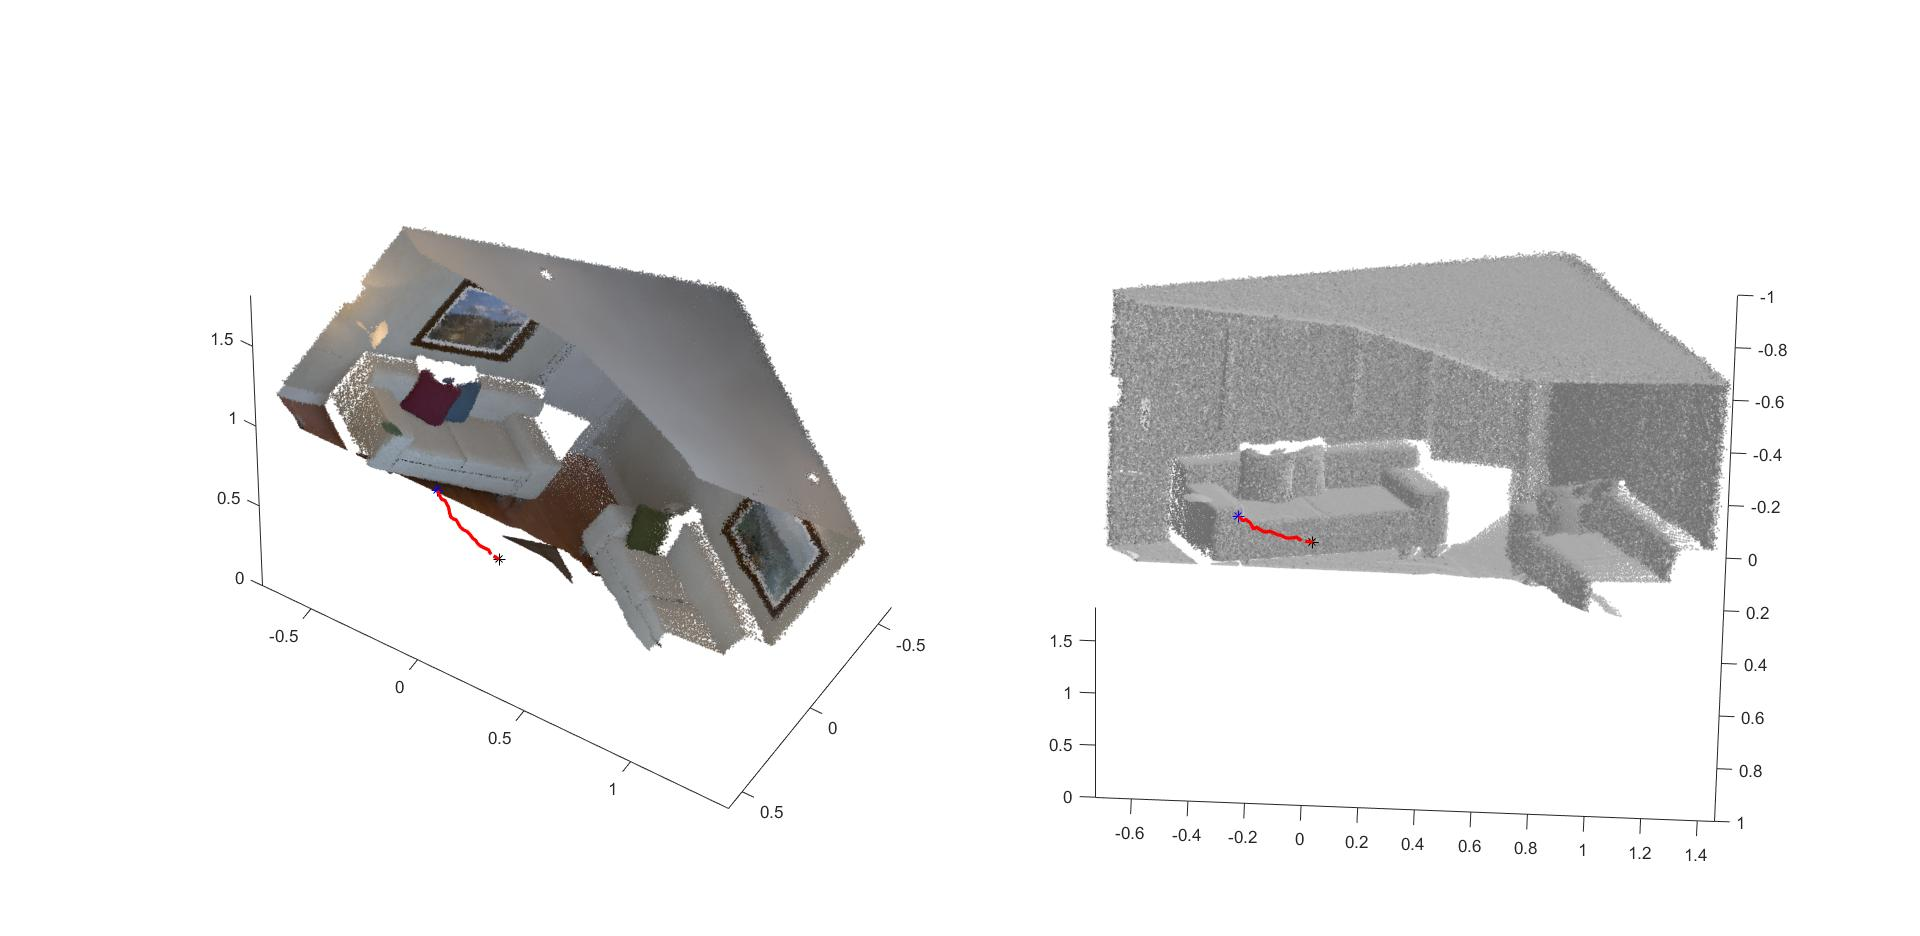
\includegraphics[width = 1.25\textwidth,center]{slam_hw3_q2_d_part1_pic2.jpg}\\ \\
	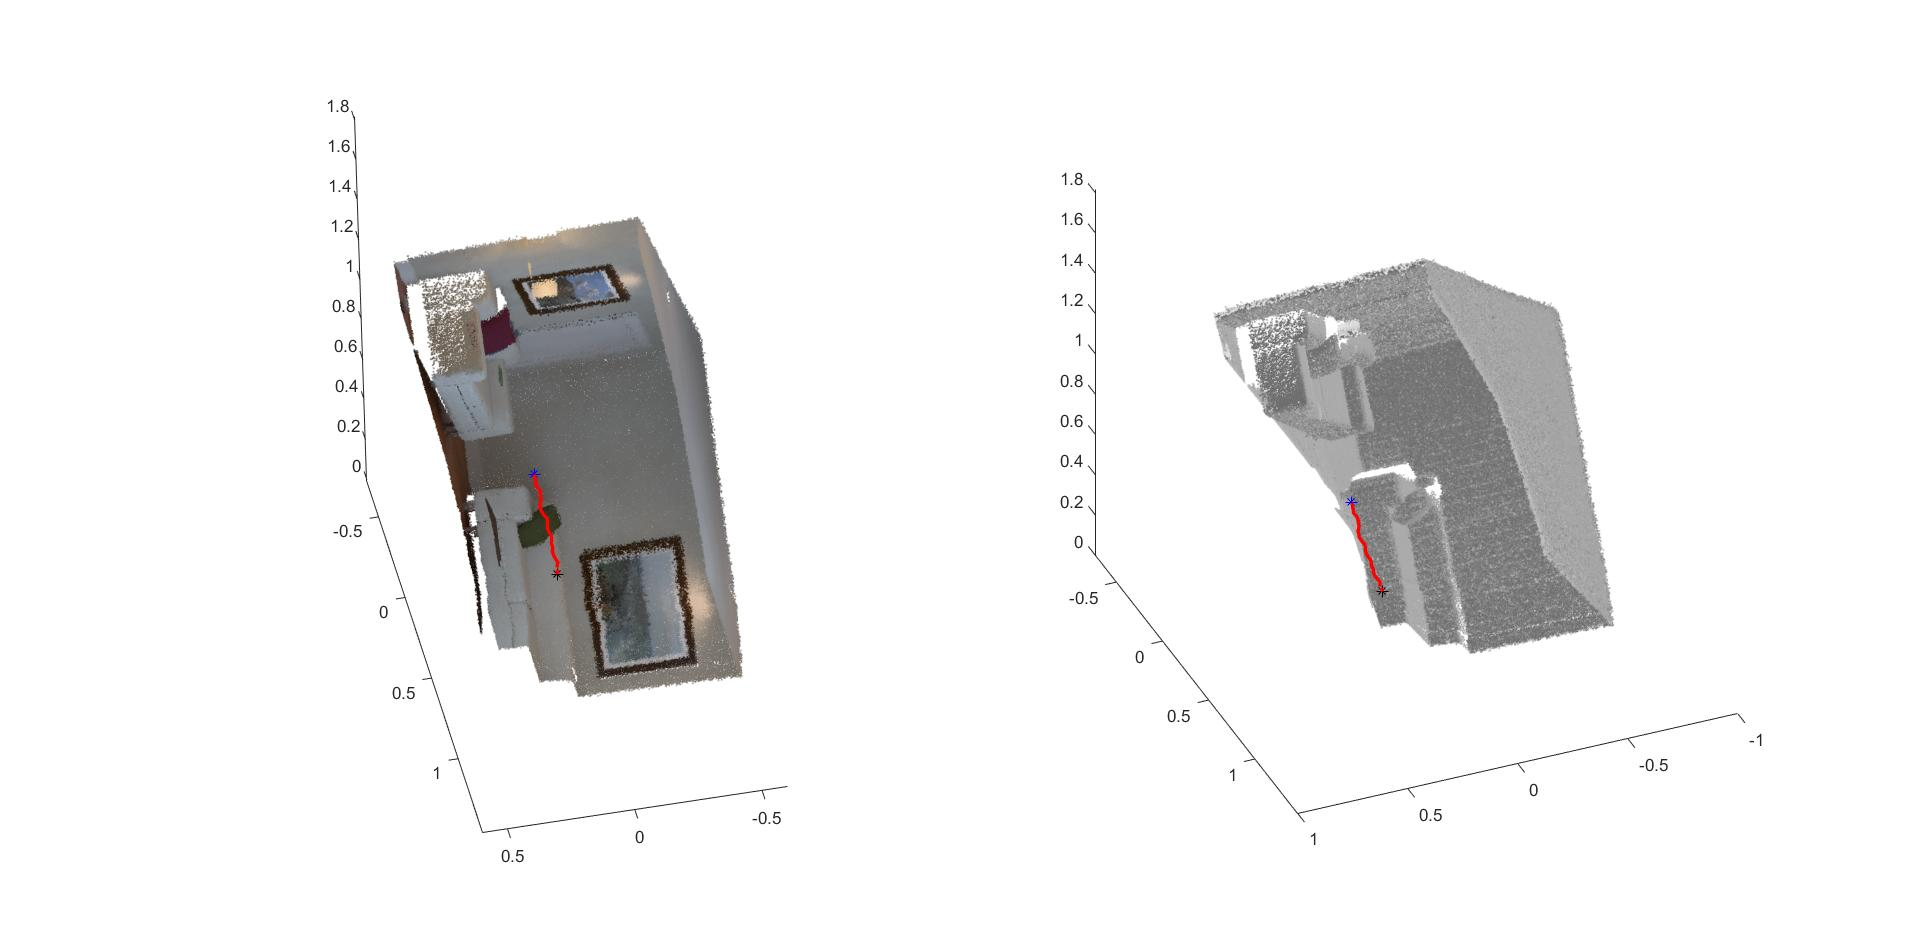
\includegraphics[width = 1.25\textwidth,center]{slam_hw3_q2_d_part1_pic3.jpg}\\ \\
	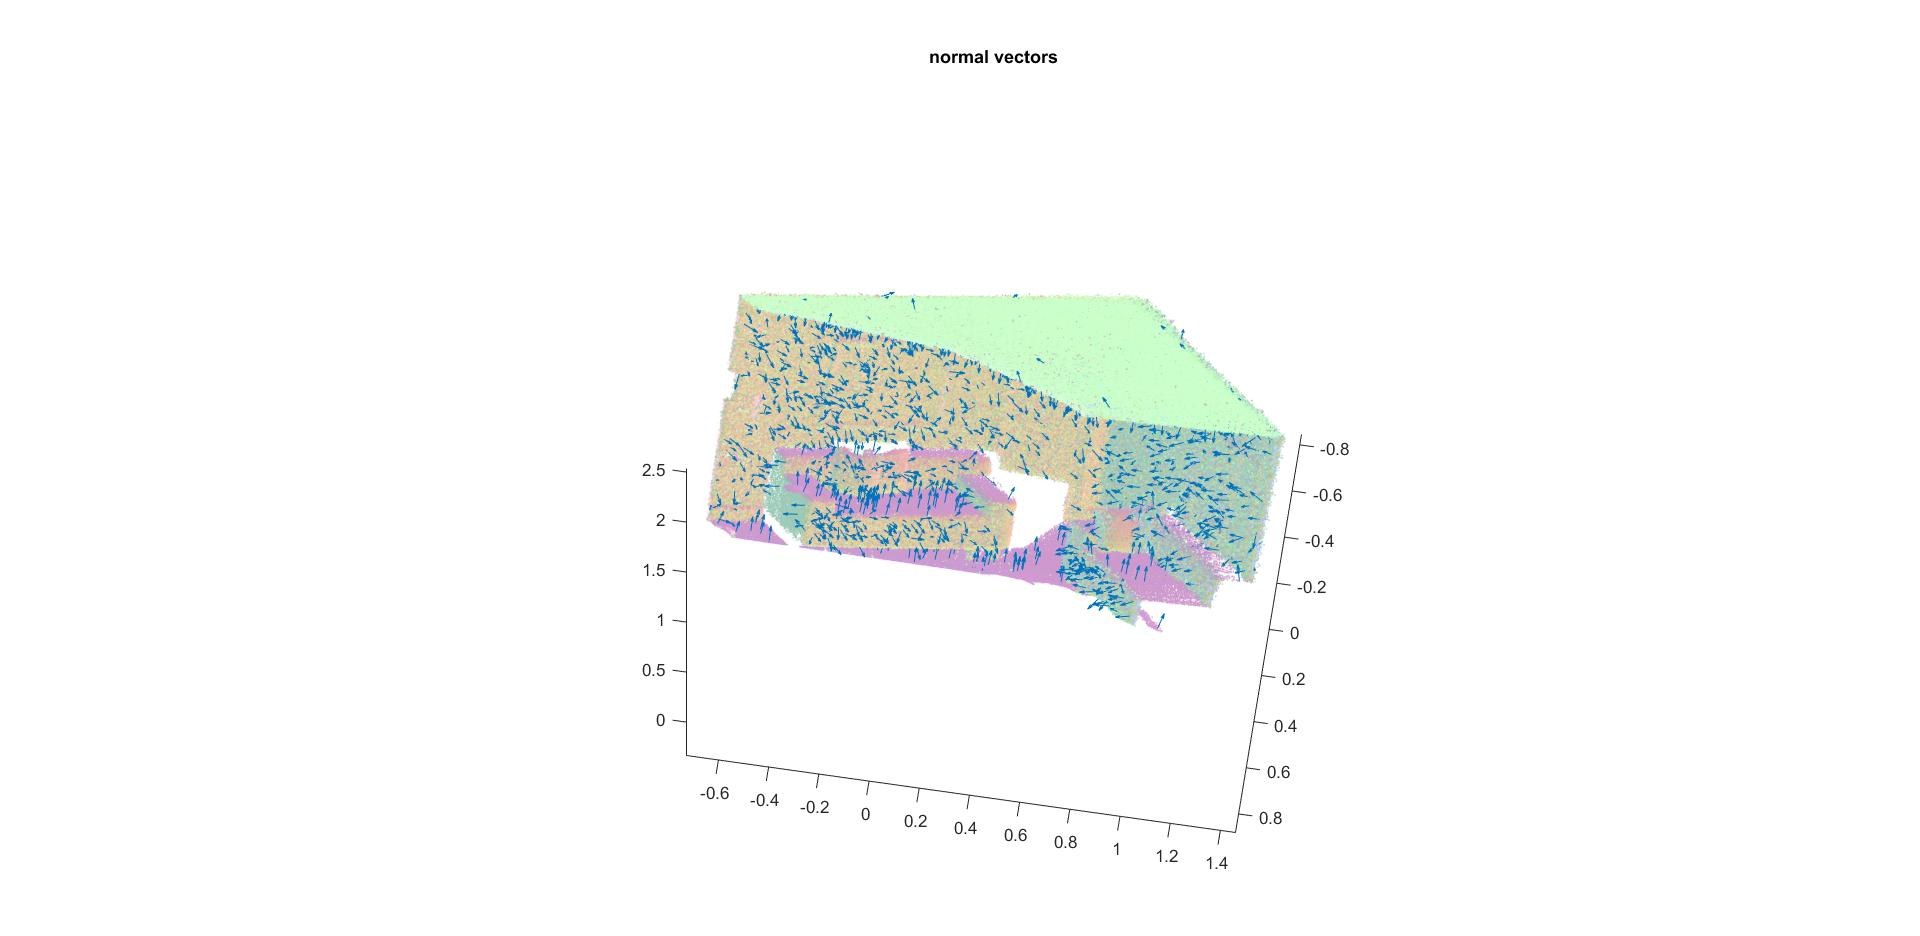
\includegraphics[width = 1.5\textwidth,center]{slam_hw3_q3_partc_normalVectors.jpg}\\ \\
	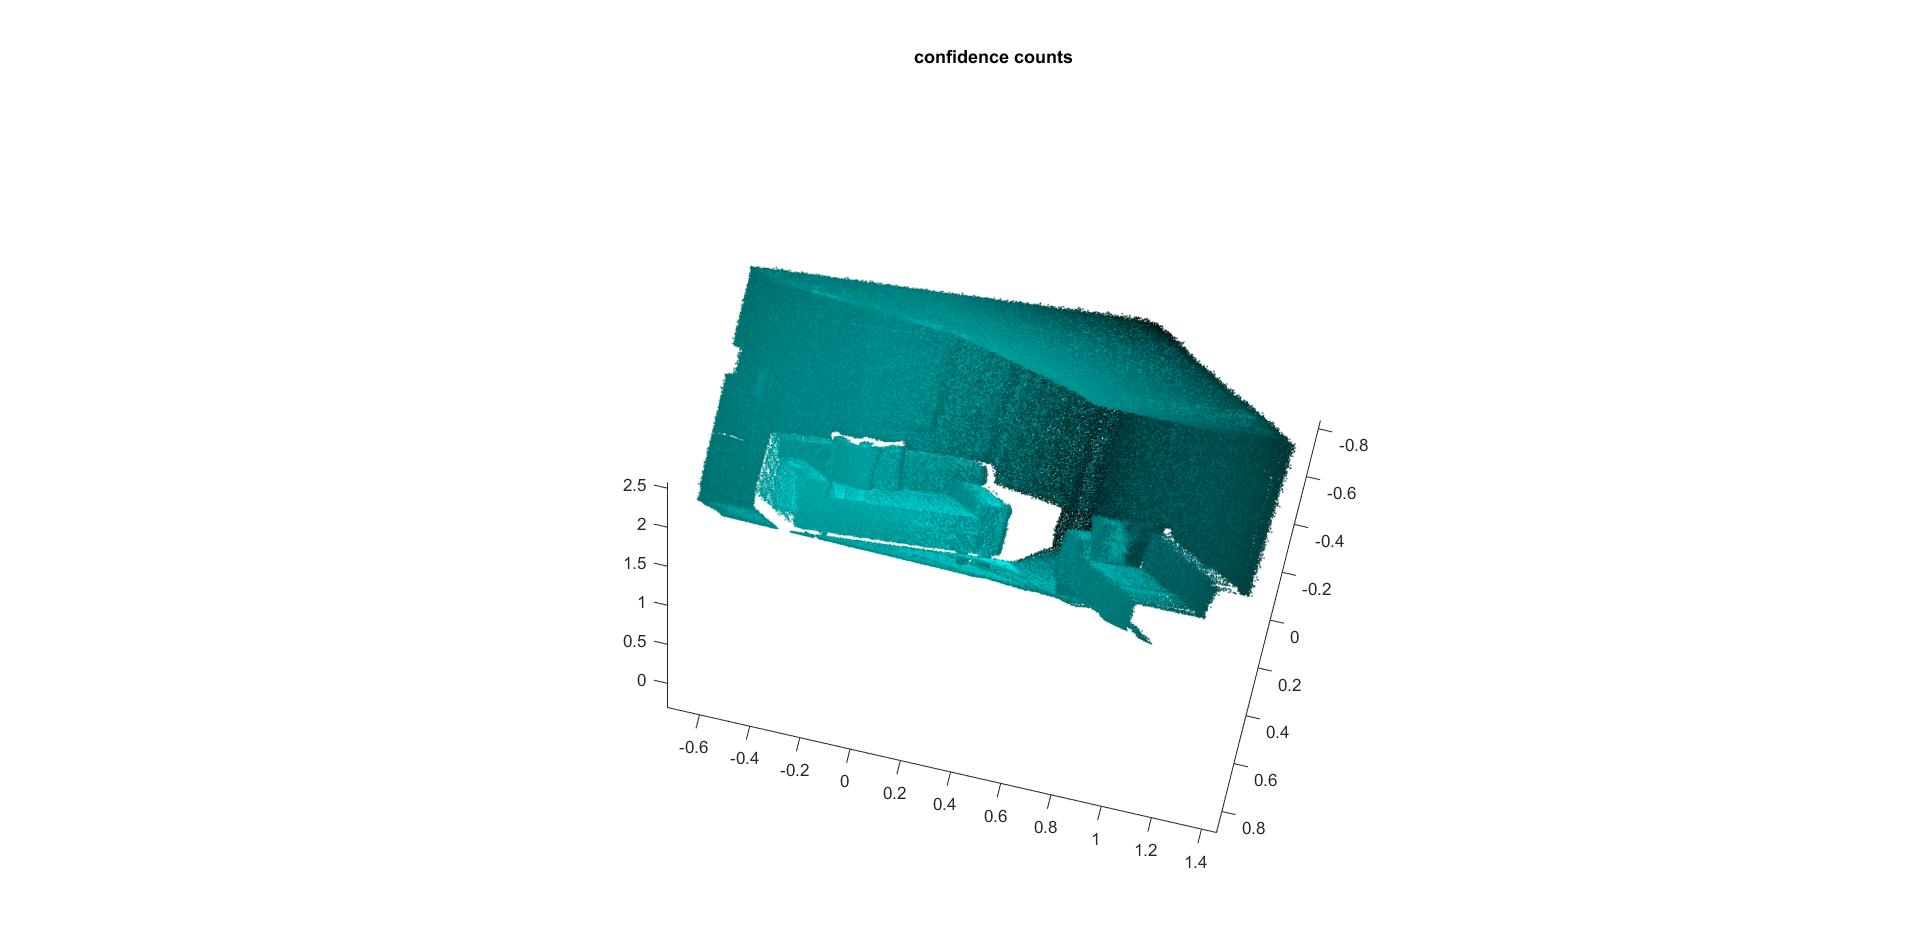
\includegraphics[width = 1.5\textwidth,center]{slam_hw3_q3_partc_confidenceCounts.jpg}\\ \\
	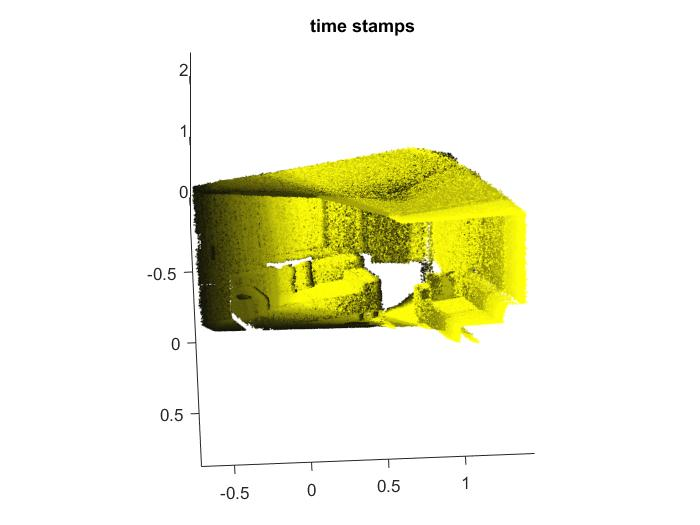
\includegraphics[width = 1.5\textwidth,center]{slam_hw3_q3_partd_timeStamps.jpg}\\ \\
	
\end{adjustwidth}

\end{document}